\documentclass[twocolumn,11pts]{IEEEtran}
\usepackage[spanish,es-lcroman,es-tabla,es-nosectiondot]{babel}
\decimalpoint
\usepackage[utf8]{inputenc}
\usepackage{csquotes}
 
\usepackage{textcomp}

\usepackage[table,xcdraw]{xcolor}
\usepackage{graphicx}
\usepackage{cite}
\usepackage{enumerate}
\usepackage{amsmath}
\renewcommand{\figurename}{Figura}
\usepackage{listings}
\usepackage{tabularx}
\usepackage{multirow}
\usepackage{colortbl}
\usepackage{booktabs}
\usepackage{graphicx}
\usepackage{amssymb}
\usepackage{url}
\usepackage{array}
\usepackage{color}
\usepackage{float}
\usepackage[american]{circuitikz}

\renewcommand{\figurename}{Figura}
\renewcommand{\refname}{Referencias}
\renewcommand{\IEEEkeywordsname}{Palabras clave}

\author{Esteban}
\title{Informe}



\renewcommand{\leftmark}{Informe Práctica No.2: Circuitos resistivos (Kirchhoff, Superposición y Thévenin) 29 de abril de 2019}

\begin{document}


\renewcommand{\tablename}{TABLA}

\title{Informe Práctica No.4: Respuesta sinusoidal de circuitos de $1^{er}$ y $2^{do}$ orden; Gr 5, Eq 4}

\author{Escobar Jaimes, Samuel Orlando$^1$; Ladino Fajardo, Esteban$^2$ \& Tamayo Perez, Ivan Leonardo$^3$    \\
Facultad de ingeniería. Universidad Nacional de Colombia. \\
Departamento de ingeniería eléctrica y electrónica.\\
\{soescobarj, eladinof, iltamayop\}@unal.edu.co}
\author{ Escobar Jaimes, Samuel Orlando$^1$; Ladino Fajardo, Esteban$^2$ \& Tamayo Perez, Ivan Leonardo$^3$.
\\\
soescobarj, eladinof, iltamayop\{@unal.edu.co\}\\
Universidad Nacional de Colombia. Facultad de ingeniería.\\
Departamento de ingeniería eléctrica y electrónica. \\
\thanks{$^{1}$
        {\small Estudiante de ingeniería eléctrica}} 
\thanks{$^{2}$
        {\small Estudiante de ingeniería electrónica}}
\thanks{$^{3}$
        {\small Estudiante de ingeniería electrónica}}
}

\maketitle
\begin{abstract}
   
\end{abstract}
\begin{IEEEkeywords} 
\end{IEEEkeywords}



%%%%%%%%%%%%%%%%%%%%%%%%%%%%%%%%%%%%%%%% Introducción
\section{Introducción}

%%%%%%%%%%%%%%%%%%%%%%%%%%%%%%%%%%%%%%%% Diseños y simulaciones


\section{Antes de Clase}


%%%%%%%%%%%%%%%%%%%%%%%%%%%%%%%%%%%%%%%% Resultados y análisis

\section{Resultados y análisis}

\subsection{Circuito RLC}
 
\section{Discusión de resultados}

%%%%%%%%%%%%%%%%%%%%%%%%%%%%%%%%%%%%%%%%%%%%%%%%%%%%%%%%%%%%% Conclusiones
\section{Conclusiones}
\begin{itemize}

\item 
\item 
\item 
\item 
\item 
\item 
\end{itemize}

%%%%%%%%%%%%%%%%%%%%%%%%%%%%%%%%%%%%%%%%%%%%%%%%%%%%%%%%%%%%% Referencias


\renewcommand{\refname}{Referencias}

\begin{thebibliography}{5}
\bibitem{1} S.Franco.(2006). Electric circuits fundamentals.
Oxford university press, (1999), pag 387.

\bibitem{2} Charles K.Alexander, Matthew.N.O Sadiku.(2006). Fundamentos de circuitos eléctricos.
Circuito. (2017, 17 de enero).
\bibitem{3} Hayt, William H., Kemmerly, Jack E. Análisis de circuitos en Ingeniería, Mc Graw Hill. Octava edición. (2012)
\end{thebibliography}



%Example de figuras

\begin{center}
 \begin{figure}[H]
 \centering
 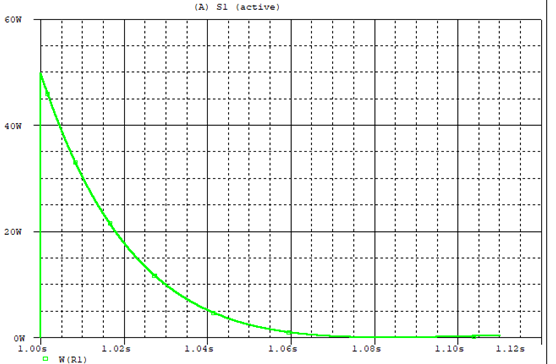
\includegraphics[scale=0.6]{Potencia1.png}
\caption{Simulación de potencia de Montaje fig.20.}
 \end{figure}
\end{center}


%Example de tabla



\begin{table}[H]
        \caption{Valores de tensión de la figura 1 }
        \label{Tabla 1}
        \begin{center}
        \begin{tabular}{|c||c||c||c||c||c|}
        \hline
        \multicolumn{6}{|c|}{Tensión Circuito 1}\\ \hline
        \multirow{ 2}{*}{Res.}& $T^a$	&Sim. & Exp. \tiny{$T_{RMS}$} & $E_{rel}$&$E_{Abs}$\\
         &  \tiny{(V)} &  \tiny{(V)} & \tiny{(V) $\pm$ 0.005} & \tiny{(\%)} & \tiny{$(v)$} \\ \hline
        \tiny{$R_1$} &3.282 & 3.28 &3.300 &0.548 & 0.018 \\  \hline
        \tiny{$R_2$} &3.152 & 3.15 &3.195 &1.377 & 0.043 \\  \hline
        \tiny{$R_3$} &0.124& 0.13 &0.104  &16.183 & 0.020 \\  \hline
        \tiny{$R_4$} &6.851 & 6.85 &6.780  &1.033 & 0.071 \\  \hline
        \tiny{$R_5$} &1.719 &1.72 &1.692  &1.586 &0.027 \\  \hline
        \end{tabular}
        \end{center}
    \end{table}
    \vspace{0.2 cm}


\begin{table}[H]
    \centering
    \caption{\textsc{\footnotesize Características de NMOS}}
    \label{Table 1}
    \begin{tabular}{@{}cccc@{}}
    \toprule
    \toprule
    R {[}$\Omega ${]} & $V_R${[}V{]} & $V_{DS}$ {[}V{]} & ID {[}$\mu A${]} \\ \midrule
    101.3  &  0.0031  &  5.097  &  31.00  \\


  221.1  &  0.0070  &  5.093  &  31.82  \\


  388  &  0.0121  &  5.088  &  31.03  \\


  504  &  0.0160  &  5.084  &  31.37  \\


  675  &  0.0214  &  5.079  &  31.47  \\


  797  &  0.0253  &  5.075  &  30.85  \\


  1015  &  0.0321  &  5.068  &  32.10  \\


  1505  &  0.0475  &  5.053  &  31.67  \\


  2670  &  0.0845  &  5.016  &  31.30  \\


  3880  &  0.1227  &  4.977  &  31.46  \\


  5000  &  0.1600  &  4.940  &  31.37  \\


  6740  &  0.2122  &  4.888  &  31.21  \\


  10060  &  0.3159  &  4.784  &  31.59  \\


  21590  &  0.6770  &  4.423  &  30.77  \\


  55500  &  1.700  &  3.400  &  30.36  \\


  67400  &  2.060  &  3.040  &  30.29  \\


  99100  &  2.982  &  2.118  &  29.82  \\


  340000  &  4.800  &  0.3000  &  14.55  \\


  564000  &  5.027  &  0.0730  &  8.977  \\


  1007000  &  5.050  &  0.0500  &  5.050  \\
    \bottomrule \bottomrule
    \end{tabular}
\end{table}




\renewcommand{\refname}{Referencias}

\begin{thebibliography}{5}
\bibitem{1} S.Franco.(2006). Electric circuits fundamentals.
Oxford university press, (1999).
\bibitem{2} Serway, Jewett,Física para ciencias e ingeniería, cencage learning, (2005).
\bibitem{3} Charles K.Alexander, Matthew.N.O Sadiku.(2006). Fundamentos de circuitos eléctricos.
Circuito. (2017, 17 de enero).
\bibitem{4} Hayt, William H., Kemmerly, Jack E. Análisis de circuitos en Ingeniería, Mc Graw Hill. Octava edición. (2012)
\end{thebibliography}

\end{document}